\tikzset{near start abs/.style={xshift=1cm}}

\begin{figure}
    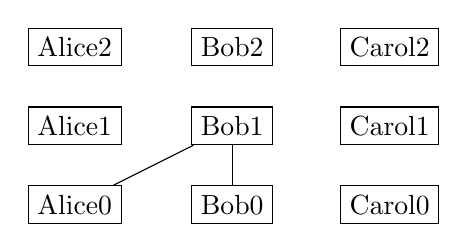
\begin{tikzpicture}
        % place nodes
        \node[draw] at (0, 0)   (a0) {Alice0};
        \node[draw] at (0, 1)   (a1) {Alice1};
        \node[draw] at (0, 2)   (a2) {Alice2};

        \node[draw] at (2, 0)   (b0) {Bob0};
        \node[draw] at (2, 1)   (b1) {Bob1};
        \node[draw] at (2, 2)   (b2) {Bob2};
        
        \node[draw] at (4, 0)   (c0) {Carol0};
        \node[draw] at (4, 1)   (c1) {Carol1};
        \node[draw] at (4, 2)   (c2) {Carol2};

        % draw edges
        \draw[] (a0) -- (b1);
        \draw[] (b0) -- (b1);
        % \draw[] (a) node[above,xshift=1cm] {$x(kT)$} -- (b);
        % \draw[] (c) node[above,xshift=1cm] {$y(kT)$} -- (d);
        % \draw (0,-3) node[above,near start abs] {Test} -- ++(7,0);
    \end{tikzpicture}

    \label{fig:hashgraph}
    \caption{
        Example of how hashgraph spreads information via gossip.
        Alice tells Bob what she knows. 
    }
\end{figure}
